\documentclass{article}
\usepackage[T1]{fontenc}
\usepackage{lmodern}
\usepackage{graphicx}
\usepackage{amsmath,amssymb}
\usepackage[a4paper,margin=2cm]{geometry}
\usepackage[absolute,overlay]{textpos}
\setlength{\TPHorizModule}{1mm}
\setlength{\TPVertModule}{1mm}
\usepackage[indonesian]{babel}
\usepackage{hyperref}
\setlength{\emergencystretch}{2em}
% unit: Halaman 68

\begin{document}

% === Halaman 68 (llm) ===

\begin{itemize}
  \item Untuk melakukan dekripsi, maka urutan komputasi di dalam Feistel dibalik (dari "bawah" ke "atas"), itulah sebabnya dinamakan \textit{reversible}.
\end{itemize}

\vspace{60mm}

Jaringan \textit{Feistel} pada dekripsi putaran ke-$i$

\begin{align*}
  R_{i-1} &= L_i \\
  L_{i-1} &= R_i \oplus f(R_{i-1}, K_i) = R_i \oplus f(L_i, K_i)
\end{align*}

% deskripsi: Diagram alur jaringan Feistel untuk proses dekripsi putaran ke-i, menunjukkan aliran data dari L_i dan R_i kembali ke L_{i-1} dan R_{i-1} dengan fungsi f dan kunci K_i.
% bbox normalisasi: [0.1180, 0.2530, 0.8100, 0.7450]
\begin{textblock*}{145.32mm}(24.78mm,75.14mm)
\noindent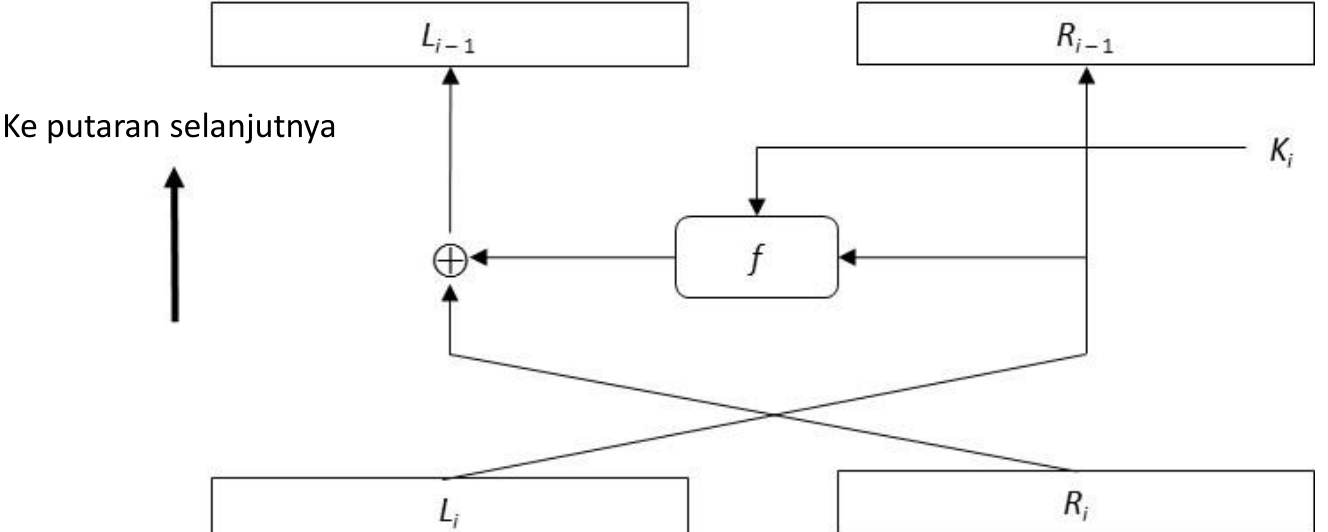
\includegraphics[width=145.32mm,height=146.12mm]{../../images/llm/page_068_img_01.png}%
\end{textblock*}

\end{document}
